\documentclass{article}
% translate with >> pdflatex -shell-escape <file>

% This file is an extract of the PGFPLOTS manual, copyright by Christian Feuersaenger.
% 
% Feel free to use it as long as you cite the pgfplots manual properly.
%
% See
%   http://pgfplots.sourceforge.net/pgfplots.pdf
% for the complete manual.
%
% Any required input files (for <plot table> or <plot file> or the table package) can be downloaded
% at
% http://www.ctan.org/tex-archive/graphics/pgf/contrib/pgfplots/doc/latex/
% and
% http://www.ctan.org/tex-archive/graphics/pgf/contrib/pgfplots/doc/latex/plotdata/

\usepackage{pgfplots}
\pgfplotsset{compat=newest}

\pagestyle{empty}

\begin{document}
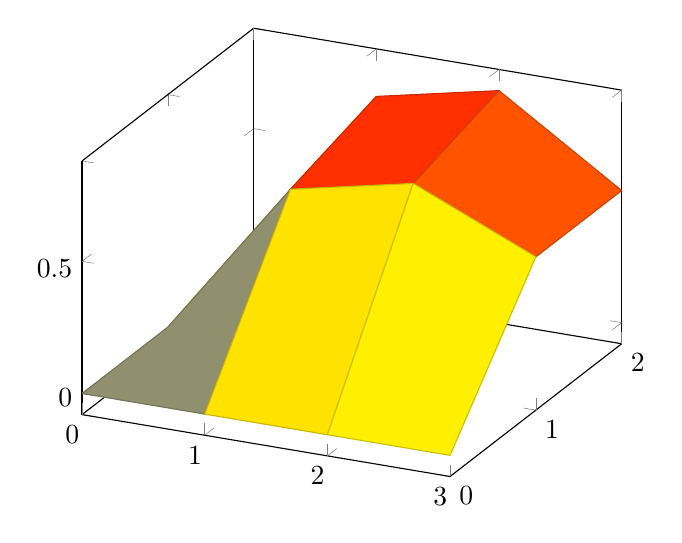
\begin{tikzpicture}
\begin{axis}[mesh/ordering=y varies]
	% this yields a 3x4 matrix in colwise ordering:
	\addplot3[surf] coordinates {
		(0,0,0) (0,1,0)   (0,2,0)

		(1,0,0) (1,1,0.6) (1,2,0.7)

		(2,0,0) (2,1,0.7) (2,2,0.8)

		(3,0,0) (3,1,0.5) (3,2,0.5)
	};
\end{axis}
\end{tikzpicture}
\end{document}
